\documentclass{report}

\usepackage{a4wide}
\usepackage{amsmath}
\usepackage{amsfonts}
\usepackage[latin1]{inputenc} %input font encoding
\usepackage[T1]{fontenc} % output font encoding
\usepackage{listings}
\usepackage{hyperref}
\usepackage[svgnames]{xcolor}

\usepackage{graphicx}
\graphicspath{{./images/}}

\usepackage{etoolbox} % Add bibliography to toc
\makeatletter
\patchcmd{\thebibliography}{%
  \chapter*{\bibname}\@mkboth{\MakeUppercase\bibname}{\MakeUppercase\bibname}}{%
  \chapter{Bibliography}}{}{}
\makeatother

\hypersetup{
    colorlinks,
    citecolor=DodgerBlue,
    filecolor=black,
    linkcolor=black,
    urlcolor=black
}

\title{Visualisation of Epidemics Simulation}
\author{Matthew Lakin\\\textbf{Supervisor: Hossein Nevisi}}
\date{October 2024 - May 2025}

\begin{document}
\maketitle
\newpage

\tableofcontents


\newpage

\chapter{Abstract}
[WILL WRITE AT END OF PROJECT]

\newpage

\chapter{Introduction}
\begin{center}
    \LARGE{"We've actually invested very little in a system to stop an epidemic. We're not ready for the next epidemic."}
\end{center}
\begin{flushright}
    \large{- Bill Gates, 2015 \cite{gates:2015}}
\end{flushright}
\vspace{0.2cm}In recent years, we have all become too familiar with viruses and epidemics. From Ebola landing in Europe and America in the 2010s after ravaging through Africa, to Covid-19 in the 2020s.\\
New epidemics seem to be springing up at a rate never seen before \cite{morandFigure} and I think there are multiple causes to this.For one, access to medicine has been a huge help in increasing survival rates for all sorts of ailments. However, this has caused complacency in the world of medicine and Antibiotic Resistance, where medicine becomes ineffective to bacterial infections, has become one of the most prevalant issues the human race will face in the coming decades.
Being able to use existing data to predict how epidemics will spread and what


Going back to the 14th Century, the Black Death, or the bubonic plague was one of the worst outbreaks in history. It killed between 75 and 200 million people in a few years time which was 30-50\% of the total population of Europe at the time \cite{dewitte2008selectivity}. 


Smallpox still remains as the only human-affecting virus which has been functionally extinct as a result of human intervention \cite{cdc:smallpox}. This was a result of a combination of mass vaccination, containment and tracking.
In this paper, I wanted to focus on the tracking aspect of containing diseases and how it can be a useful tool to not only teach us about what happened previously, but to predict and forecast what could happen in the future. \\ \\
\textbf{This whole section will be rewritten at the end of the project. I will be able to give a more accurate introduction to the project once I have completed it.}\\

\newpage

\chapter{Problem Domain}
\section{Minimum Viable Product}
I have identified the minimal requirements for this project to be successful.
\begin{enumerate}
    \item The dashboard must show a map of the Earth.
    \item The dashboard must visualise the COVID-19 data and show the number of global cases and deaths per week.
    \item The map will render polygon and country data from a GeoJSON file.
    \item The individual countries must be clickable.
    \begin{enumerate}
        \item Clicking a country will send the user to a new page.
        \item The new page will show the number of cases and deaths per week.
        \item The new page will show a graph of the number of cases and deaths per week. 
    \end{enumerate}
    \item The dashboard must show a timeline of the epidemic.
    \begin{enumerate}
        \item The timeline will be a slider.
        \item The user must be able to scrub through the timeline.
        \item The timeline will show the current week.
    \end{enumerate}
    \item The user must be able to select data from a file to be displayed.
    \begin{enumerate}
        \item The code will accept a clean JSON file.
        \item The JSON file will have the same format as the COVID-19 data.
    \end{enumerate}
\end{enumerate}
\newpage
\section{Stretch Goals}
For this project, the following aspirational requirements have been identified:
\begin{enumerate}
    \item Zooming in on the map.
    \begin{itemize}
        \item This is my most realistic stretch goal. It would require using a library to render the map and allow the user to zoom in and out.
    \end{itemize}
    \item Hotspots on the map.
    \begin{itemize}
        \item This would require analysis of the data to find out where the rate of infection is highest.
    \end{itemize}
    \item Analysis of data with other data sources to search for correlations.
    \begin{itemize}
        \item I am currently unsure what data sources I would use for this, but it would be interesting to see if there are any correlations between the spread of the virus and other factors.
    \end{itemize}
    \item Predictctive modelling and forecasting.
    \begin{itemize}
        \item This is my most ambitious stretch goal. I would like to be able to predict the spread of the virus using the data I have. This would require a lot of work and research into the field of predictive modelling. This would likely be a separate project in itself.
    \end{itemize}
\end{enumerate}
\newpage

\chapter{Methodology}
For this project I will incorperate a Waterfall model into my project since it will ensure my code and report as a whole is developed in a structured and ordered fashion.\\
The steps of Waterfall I will be following are:
\begin{enumerate}
    \item \textbf{\large{Requirements}}
    \begin{itemize}
        \item This section requires producing and refining a set of requirements. I plan on having 2 groups of requirements: Minimum Viable Product requirements and Stretch requirements.
        \item I plan on refining all the requirements in this stage so I can stay on this path plan.
    \end{itemize}
    \item \textbf{\large{Analysis}}
    \begin{itemize}
        \item In this section, I will be doing research into the problems which are discovered by my requirement refinement. I will investigate papers and other relevant published sources.
        \item I also want to investigate node packages to represent my data graphically. (This would continue into the design section)
        \item This section will likely take up a large section of my report, and I may return to this section midway through the project.
    \end{itemize}
    \item \textbf{\large{Design}}
    \begin{itemize}
        \item I would be designing the layout and colour scheme of my application as it would appear in a browser window. It is worth noting that different size screens would render it differently, so I need to take that into account when planning.
        \item I am not using a database for this project, but I will be using JSON and creating a standard design for objects in JSON will be beneficial.
        \item I need to decide what values I use for graphs and what kind of graphs to use.
    \end{itemize}
    \item \textbf{\large{Coding}}
    \begin{itemize}
        \item I will be making a web application with node.js. This will require me to create a valid work environment and get the node runtime working on my local machine. I will likely use Docker for this since it is a very easy to work with tool perfect for this application.
        \item I will mostly be using TypeScript for this project because of type safety and native compatibility with web development. There will also be HTML and CSS for loading the TS canvas and aligning elements.
        \item Node.js also comes with node package manager which will also be useful for loading the custom packages I plan on using in this project.
    \end{itemize}
    \item \textbf{\large{Testing}}
    \begin{itemize}
        \item For testing, I will be using a variety of normal, boundary and erroneous tests to check my software for crashes, unexpected results, and vulnerabilities. Using a type-safe language like TypeScript intends to minimise the chances of these happening.
        \item I also plan on having 3rd-party applicants to test my application. They would have a list of things to do in the application so I can analyse the ease of use.
        \item I would also ask them to fill in a questionnaire.
    \end{itemize}
    \item \textbf{\large{Operations}}
    \begin{itemize}
        \item I want to deploy my application to a server hosted by the university.
        \item Node.js applications are commonly deployed onto servers and having a production repository would be a good standard for myself. Pushing to a server from a local git repository is a highly transferable skill which is widely used. Test
    \end{itemize}
\end{enumerate}
\section{Gantt Chart}
    \begin{center}
        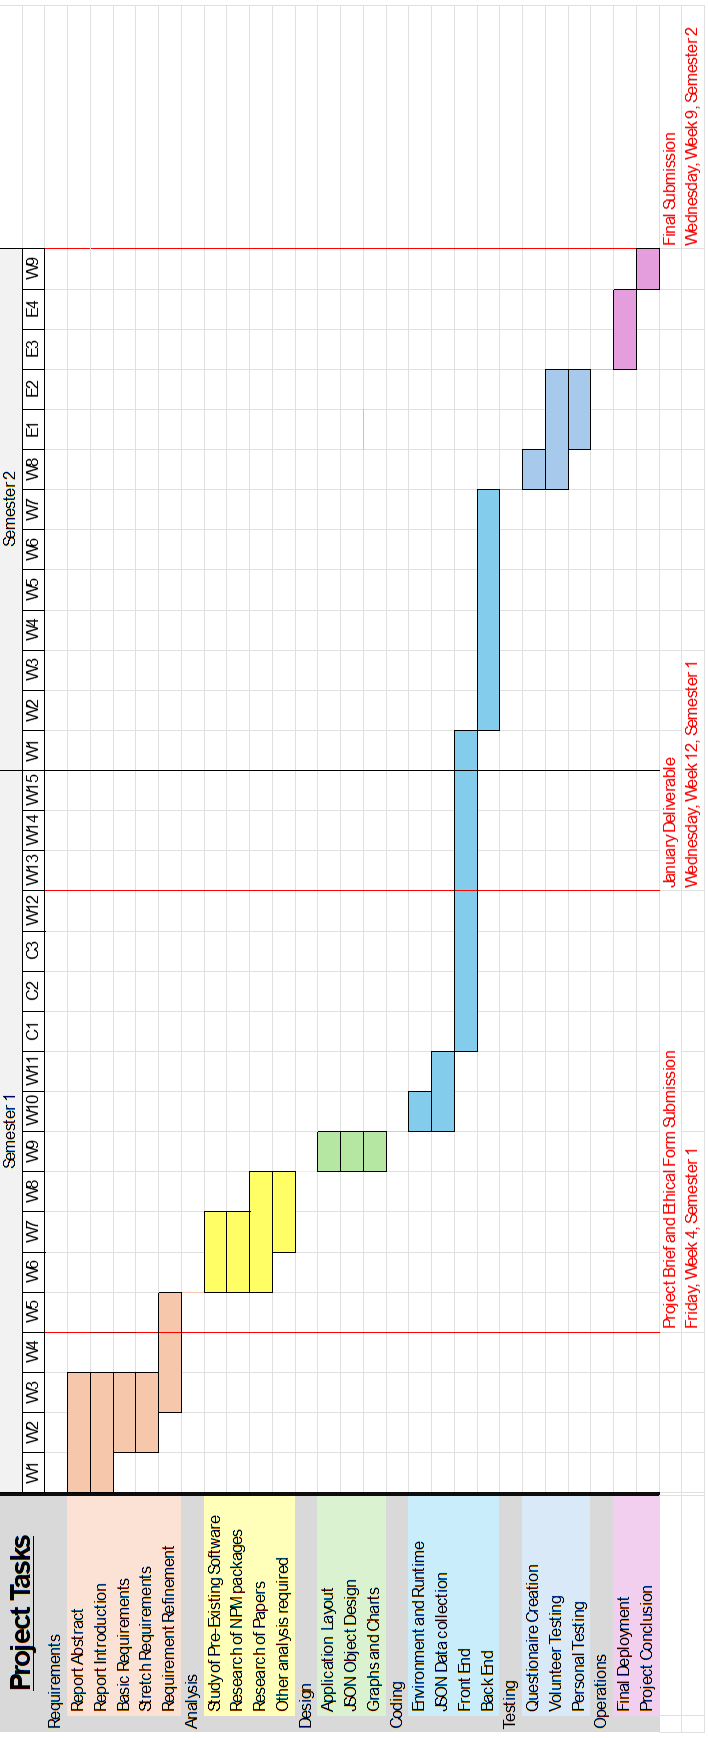
\includegraphics[height=0.95\textheight]{gantt_chart}
    \end{center}

\newpage

\newpage

\chapter{Research}
\section{Existing Solutions}
\subsection{COVID-19 Dashboard}
A common tool for data visualisation is a software called PowerBI, a Microsoft product which allows for the creation of dashboards. 
The dashboard in the figure shows a real-time representation of the COVID-19 pandemic.
\begin{center}
    \begin{figure}[h]
        \centering
        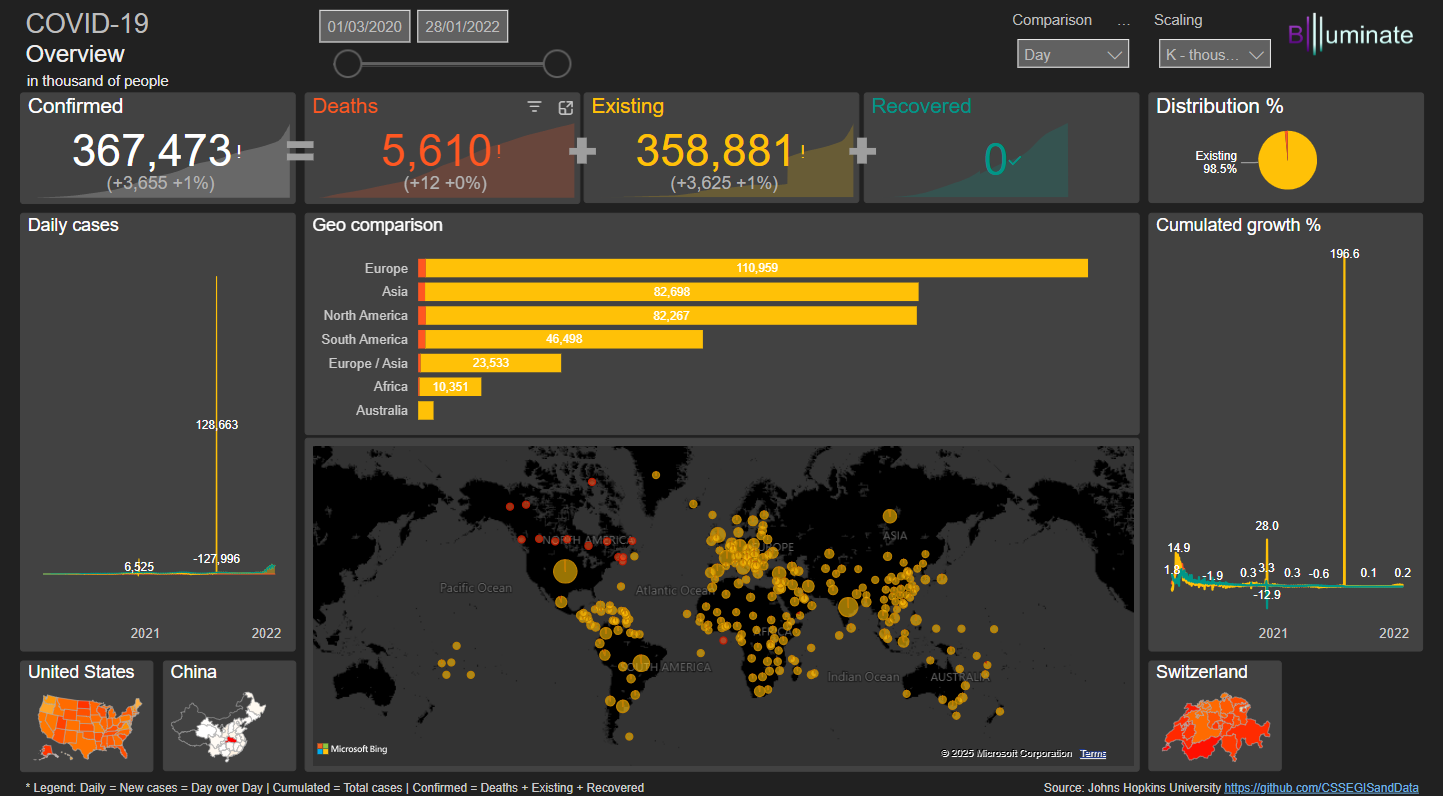
\includegraphics[width=0.95\textwidth]{PowerBI Example.png}
        \caption{COVID-19 Dashboard Example}
        \label{fig:covid19_dashboard}
    \end{figure}
\end{center}

This dashboard has a lot of information on it even at first glance. The map uses bubbles to denote hotspots of activity for the virus. The bubbles are sized by the number of cases in that country. The bubbles can also be clicked for more detailed information on that country. \\
The user is also able to alter the time frame of the data, and the data is updated in real time.\\
There is a lot here which I would like to incorperate into my own project. The map is a good way to visualise the data and the bubbles are a good way to show the number of cases in each country. I also like the big bold text which summarises the data which is easy to read.\\
\newpage
\subsection{Plague Inc.}
Plague Inc. is a game published in 2012 by Ndemic Creations. It gives the user the ability to create and spread a virus across the world. The game was initially released on mobile devices and has since been released on PC and console.\\
Mobiles games require accessible and easy to use interfaces, which is why Plague Inc. is a good example of a visual epidemic simulation. The game is simple to use and has a lot of information on the screen at once.
\begin{center}
    \begin{figure}[h]
        \centering
        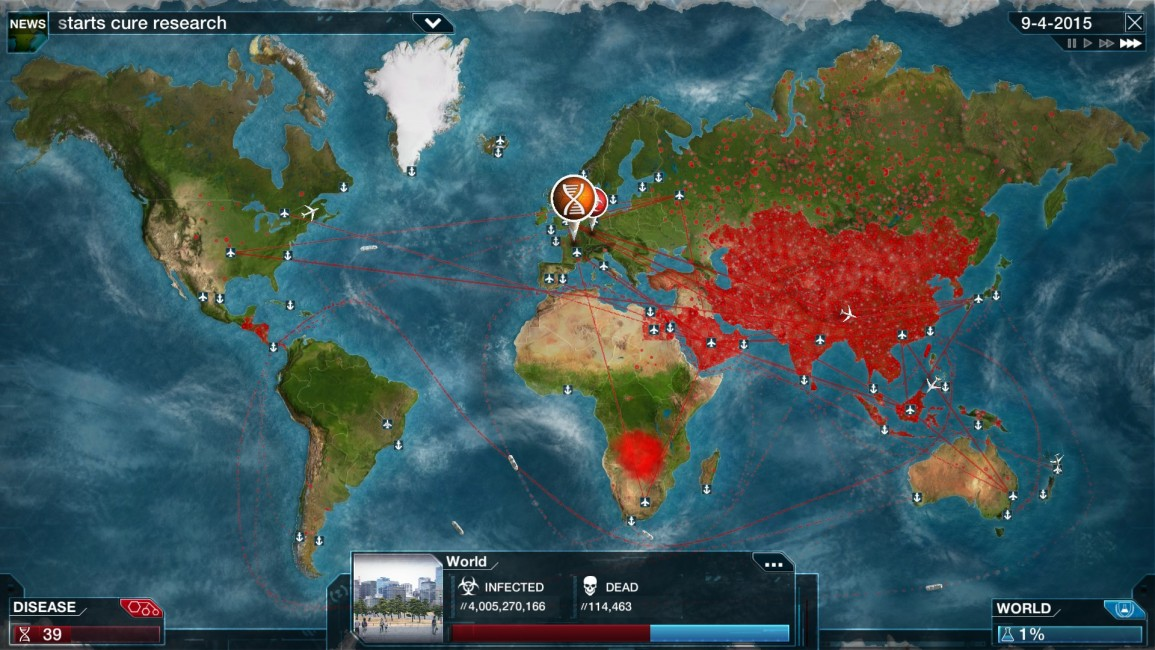
\includegraphics[width=0.95\textwidth]{Plague Inc Example.jpeg}
        \caption{Plague Inc. Dashboard Example}
        \label{fig:plagueinc_dashboard}
    \end{figure}
\end{center}
Despite many systems being dramatised for the sake of gameplay, the game offers many features which could be useful for a real-world epidemic simulation. \\
The game uses a world map which gradually changes colour as the virus spreads, this is from many red dots appearing on the map. The user also has access to individual breakdowns of each country and can see the number of cases and deaths in each country.\\ 
The game also has a transmission system which changes from coutnry to country. 
\\ \\
There is certain information provided in these examples that I will not be able to provide in my project. For example, the COVID-19 dashboard has real-time data, which I will not be able to provide. The Plague Inc. game has a transmission system which changes from country to country, which I will not be able to provide.\\

\newpage
\section{Visualisation}
\subsection{Covid-19 Data Sources}
The data for this project will be sourced from the European Centre for Disease Prevention and Control (ECDC) \cite{ecdc}. The data is historic and only has data from the 1st week of 2020 to the 23rd week of 2022. The data is in a JSON format and includes the number of cases and deaths per week for each country. The format of the data is as follows:

\begin{minipage}{0.45\textwidth}
\begin{lstlisting}[caption={Cases JSON Example}]
{
    "country": "Afghanistan",
    "country_code": "AFG",
    "continent": "Asia",
    "population": 38928341,
    "indicator": "cases",
    "weekly_count": 1368,
    "year_week": "2020-47",
    "rate_14_day": 6.5043,
    "cumulative_count": 44771,
    "source": "Epidemic
    intelligence national data"
}
\end{lstlisting}
\end{minipage}
\hfill
\begin{minipage}{0.45\textwidth}
\begin{lstlisting}[caption={Deaths JSON Example}]
{
    "country": "Afghanistan",
    "country_code": "AFG",
    "continent": "Asia",
    "population": 38928341,
    "indicator": "deaths",
    "weekly_count": 69,
    "year_week": "2020-47",
    "rate_14_day": 3.3395,
    "cumulative_count": 1695,
    "source": "Epidemic
    intelligence national data"
}
\end{lstlisting}
\end{minipage}
This is the format that the ECDC provide, but I will be ammending it slightly to make it easier to work with. I will be combining the cases and deaths into one object and adding a date field. This will make it easier to work with the data in the front end.\\
It also needs to correspond with the GeoJSON data I will be using to render the map. \\
It is worth noting that I don't want this code to be limited to just COVID-19 data. I want to be able to use this code for any epidemic data. This is why I am making the data more generic and easier to work with.
\subsection{D3.js}
D3.js is a JavaScript library for producing dynamic, interactive data visualisations in web browsers. It makes use of the widely supported SVG format to render graphics. D3.js is a powerful tool for creating visualisations and is widely used in industry.\\
D3.js is a good choice for this project as it natively supports GeoJSON data which is the format I will be using for the map. \cite{geojsonvectormaps}\\
This is exclusively used on a web browser, so I will be using node.js to serve the data to the front end.\\ \\
The GeoJSON data has much more information than the COVID-19 data. It includes geometry of the country, information regarding the countries economy, sovereign status, GDP, all in multiple languages. I will be cleaning the data to only include relevant information for this project: country name in English, country code (to link the data with the Covid-19 JSON file) and geometry information. \\
\newpage
\section{Compartmental Models}
\subsection{SIR Model}
Compartmental models are a type of mathematical model used to represent the different populations in a system. The most common compartmental system in epidemiology is the SIR model \cite{beckley2013modeling}.\\
The SIR model is a simple model which divides the population into three compartments: Susceptible, Infected and Recovered. The model is represented by the following differential equations:
\begin{align}
\frac{dS}{dt} &= -\alpha SI \label{sir_model_dS} \\
\frac{dI}{dt} &= \alpha SI - \beta I \label{sir_model_dI} \\
\frac{dR}{dt} &= \beta I \label{sir_model_dR}
\end{align}
Where:
\begin{itemize}
    \item S is the number of susceptible individuals.
    \item I is the number of infected individuals.
    \item R is the number of recovered individuals.
    \item $\alpha$ is the rate of infection.
    \item $\beta$ is the rate of recovery.
\end{itemize}
To explain this model, it's important to understand proportional reasoning. In the first equation, \ref{sir_model_dS}, the rate of change of the susceptible population is proportional to the complement of the product of the susceptible and infected populations.\\
A way to think of why that is true is because the more infected people there are, the more likely it is for a susceptible person to become infected.\\
This model is a good starting point for undestanding the spread of a virus, but it has some limitations. In this model, once you have recovered, you are no longer able to be infected. Another issue is that the model assumes the disease is non-fatal.

\subsection{Solution to the SIR Model}
The SIR model can be solved using numerical methods. The most common method is the Euler method. The Euler method is a simple method for solving ordinary differential equations. It is not the most accurate method, but it is easy to implement. The Euler method is represented by the following equations:
\begin{align}
S_{n+1} &= S_n - \alpha S_n I_n \Delta t \label{sir_euler_S} \\
I_{n+1} &= I_n + \alpha S_n I_n \Delta t - \beta I_n \Delta t \label{sir_euler_I} \\
R_{n+1} &= R_n + \beta I_n \Delta t \label{sir_euler_R}
\end{align}
Where:
\begin{itemize}
    \item $S_n$ is the number of susceptible individuals at time $n$.
    \item $I_n$ is the number of infected individuals at time $n$.
    \item $R_n$ is the number of recovered individuals at time $n$.
    \item $\Delta t$ is the time step.
\end{itemize}
If we look at the phase space of the SIR model, we can see that the model has a fixed point at the origin. This means that the model will always return to the origin. This is not the case in real life, as the disease will eventually die out. This is because the model does not take into account the finite population size.\\

\subsection{Improvements to the SIR Model}
The SIR model can be improved by adding more compartments to the model. However, this makes the model more complex and harder to solve.
\subsubsection{SEIR Model}
This model adds an exposed compartment to the SIR model. For individuals who have been infected but are not yet infectious. The model is represented by the following differential equations:
\begin{align}
\frac{dS}{dt} &= \mu N - \mu S - \frac{\beta IS}{N} \label{seir_model_dS} \\
\frac{dE}{dt} &= \frac{\beta IS}{N} - (\mu + a)E \label{seir_model_dE} \\
\frac{dI}{dt} &= aE - (\mu + \gamma)I \label{seir_model_dI} \\
\frac{dR}{dt} &= \gamma I - \mu R \label{seir_model_dR}
\end{align}
The SEIR model is better for simulations than the SIR model since it takes into account the incubation period of the disease. This is important as it is possible for a person to be infected but not yet infectious.\\
It is beyond the scope of this project to go into detail about the SEIR model, but it is worth noting that the model is more complex and requires more data to solve. The model is also more accurate than the SIR model.


\chapter{Technical Solution}

\newpage

\chapter{Results and Analysis}
\newpage

\chapter{Conclusion}
\newpage

\bibliographystyle{plain} % We choose the "plain" reference style
\bibliography{refs} % Entries are in the refs.bib file


\newpage

\chapter{Appendix}

\newpage




\end{document}